%
%   Prof. Dr. Julian Reichwald
%   auf Basis einer Vorlage von Prof. Dr. Jörg Baumgart
%   DHBW Mannheim
%
%
%	ACHTUNG: Für das Erstellen des Literaturverzeichnisses wird das modernere Paket biblatex
%			 in Kombination mit biber verwendet -- nicht mehr das ältere BibTex!
% 			 Bitte stellen Sie ggf. Ihre TeX-Umgebung
% 			 entsprechend ein (z.B. TeXStudio: Einstellungen --> Erzeugen --> Standard Bibliographieprogramm: biber)
%

\documentclass[
	12pt,
	BCOR=5mm,
	DIV=12,
	headinclude=on,
	footinclude=off,
	parskip=half,
	bibliography=totoc,
	listof=entryprefix,
	toc=listof,
	pointlessnumbers,
	plainfootsepline,
	headings=optiontohead]{scrreprt}


%	Konfigurationsdatei einziehen
% !TEX root =  master.tex

%		LANGUAGE SETTINGS AND FONT ENCODING 
%
\usepackage[ngerman]{babel} 	% German language
\usepackage[utf8]{inputenc}
\usepackage{eurosym} % Euro symbol 
\usepackage[german=quotes]{csquotes} 	% correct quotes using \enquote{}
\usepackage[T1]{fontenc}
\usepackage{amssymb} % Mathe-Package
\usepackage{pdfpages} % for appendix pdfs


%\usepackage[english]{babel}   % For english language
%\usepackage{csquotes} 	% Richtiges Setzen der Anführungszeichen mit \enquote{}

% 		HYPERREF
%
\usepackage[
hidelinks=true % keine roten Markierungen bei Links
]{hyperref}

% Zwei eigene Befehle zum Setzen von Autor und Titel. Ausserdem werden die PDF-Informationen richtig gesetzt.
\newcommand{\TitelDerArbeit}[1]{\def\DerTitelDerArbeit{#1}\hypersetup{pdftitle={#1}}}
\newcommand{\AutorDerArbeit}[1]{\def\DerAutorDerArbeit{#1}\hypersetup{pdfauthor={#1}}}
\newcommand{\Firma}[1]{\def\DerNameDerFirma{#1}}
\newcommand{\Kurs}[1]{\def\DieKursbezeichnung{#1}}

\newcommand{\DieFachrichtungDerAusbildung}[1]{\def\DieFachrichtungDerAusbildung{#1}\hypersetup{pdftitle={#1}}}
\newcommand{\DieBerufsausbildung}[1]{\def\DieBerufsausbildung{#1}\hypersetup{pdfauthor={#1}}}

% Correct superscripts 
\usepackage{fnpct}


%		CALCULATIONS
%
\usepackage{calc} % Used for extra space below footsepline



%		BIBLIOGRAPHY SETTINGS
%

% Uncomment the next three lines for author-year-style with footnotes (Chicago)
\usepackage[backend=biber, autocite=footnote, style=authoryear, dashed=false]{biblatex} 	%Use Author-Year-Cites with footnotes
\AdaptNoteOpt\footcite\multfootcite   %will add  separators if footcite is called multiple consecutive times 
\AdaptNoteOpt\autocite\multautocite % will add  separators if autocite is called multiple consecutive times

% Uncomment the next line for IEEE-style 
% \usepackage[backend=biber, autocite=inline, style=ieee]{biblatex} 	% Use IEEE-Style (e.g. [1])

% Uncomment the next line for alphabetic style 
% \usepackage[backend=biber, autocite=inline, style=alphabetic]{biblatex} 	% Use alphabetic style (e.g. [TGK12])

% Uncomment the next two lines vor Harvard-Style 
%\usepackage[backend=biber, style=apa]{biblatex} 	
%\DeclareLanguageMapping{german}{german-apa}


\DefineBibliographyStrings{ngerman}{  %Change u.a. to et al. (german only!)
	andothers = {{et\,al\adddot}},
}

%%% Uncomment the following lines to support hard URL breaks in bibliography 
%\apptocmd{\UrlBreaks}{\do\f\do\m}{}{}
%\setcounter{biburllcpenalty}{9000}% Kleinbuchstaben
%\setcounter{biburlucpenalty}{9000}% Großbuchstaben


\setlength{\bibparsep}{\parskip}		%add some space between biblatex entries in the bibliography
\addbibresource{bibliography.bib}	%Add file bibliography.bib as biblatex resource


%		FOOTNOTES 
%
% Count footnotes over chapters
\usepackage{chngcntr}
\counterwithout{footnote}{chapter}

%	ACRONYMS
%%%
%%% WICHTIG: Installieren Sie das neueste Acronyms-Paket!!!
%%%
\makeatletter
\usepackage[printonlyused]{acronym}
\@ifpackagelater{acronym}{2015/03/20}
{%
	\renewcommand*{\aclabelfont}[1]{\textbf{\textsf{\acsfont{#1}}}}
}%
{%
}%
\makeatother

%		LISTINGS
\usepackage{listings}	%Format Listings properly
\renewcommand{\lstlistingname}{Quelltext}
\renewcommand{\lstlistlistingname}{Quelltextverzeichnis}
\lstset{numbers=left,
	numberstyle=\tiny,
	captionpos=b,
	basicstyle=\ttfamily\small,
	commentstyle=\itshape,
	breaklines=true, 
	breakatwhitespace=true,
	showstringspaces=false,
	escapeinside={@@},
	keywordstyle=\bfseries,
	postbreak=\raisebox{0ex}[0ex][0ex]{\ensuremath{\hookrightarrow\space}}
}

%LISTING inline a tabular/table
\newcommand\tablstinline[2][]{\lstinline[#1]{#2}}

% LISTINGS: eigene Programmiersprache; bei morekeywords die zusätzlichen einfügen
\lstdefinelanguage{PLSQL}{
	language     = SQL,
	morekeywords = {over, partition}}

% ---- LISTING FOR YAML FILES ----
%\usepackage[dvipsnames]{xcolor}
%\usepackage{listings}
\usepackage{color}
\newcommand\YAMLcolonstyle{\color{red}\mdseries}
\newcommand\YAMLkeystyle{\color{black}\bfseries}
\newcommand\YAMLvaluestyle{\color{black}\mdseries}

\makeatletter

% here is a macro expanding to the name of the language
% (handy if you decide to change it further down the road)
\newcommand\language@yaml{yaml}

\expandafter\expandafter\expandafter\lstdefinelanguage
\expandafter{\language@yaml}
{
	keywords={true,false,null,y,n},
	keywordstyle=\color{darkgray}\bfseries,
	basicstyle=\YAMLkeystyle,                                 % assuming a key comes first
	sensitive=false,
	comment=[l]{\#},
	morecomment=[s]{/*}{*/},
	commentstyle=\color{purple}\ttfamily,
	stringstyle=\YAMLvaluestyle\ttfamily,
	moredelim=[l][\color{orange}]{\&},
	moredelim=[l][\color{magenta}]{*},
	moredelim=**[il][\YAMLcolonstyle{:}\YAMLvaluestyle]{:},   % switch to value style at :
	morestring=[b]',
	morestring=[b]",
	literate =    {---}{{\ProcessThreeDashes}}3
	{>}{{\textcolor{red}\textgreater}}1     
	{|}{{\textcolor{red}\textbar}}1 
	{\ -\ }{{\mdseries\ -\ }}3,
}

% switch to key style at EOL
\lst@AddToHook{EveryLine}{\ifx\lst@language\language@yaml\YAMLkeystyle\fi}
\makeatother

\newcommand\ProcessThreeDashes{\llap{\color{cyan}\mdseries-{-}-}}
% --------------------------

%		EXTRA PACKAGES
\usepackage{lipsum}    %Blindtext
\usepackage{graphicx} % use various graphics formats
\usepackage[german]{varioref} 	% nicer references \vref
\usepackage{caption}	%better Captions
\usepackage{booktabs} %nicer Tabs
\newcommand{\ra}[1]{\renewcommand{\arraystretch}{#1}}
\usepackage{longtable} %multipages booktabs
\usepackage{array}
%\newcolumntype{P}[1]{>{\raggedright\arraybackslash}p{#1}}


%		ALGORITHMS
\usepackage{algorithm} %float wrapper for algorithms.
\usepackage{algpseudocode}
\renewcommand{\listalgorithmname}{Algorithmenverzeichnis }
\floatname{algorithm}{Algorithmus}


%		FONT SELECTION: Entweder Latin Modern oder Times / Helvetica
\usepackage{lmodern} %Latin modern font
%\usepackage{mathptmx}  %Helvetica / Times New Roman fonts (2 lines)
%\usepackage[scaled=.92]{helvet} %Helvetica / Times New Roman fonts (2 lines)

%		PAGE HEADER / FOOTER
%	    Warning: There are some redefinitions throughout the master.tex-file!  DON'T CHANGE THESE REDEFINITIONS!
%\RequirePackage[automark,headsepline,footsepline]{scrpage2}
\RequirePackage[automark,headsepline,footsepline]{scrlayer-scrpage}
\pagestyle{scrheadings}
\renewcommand*{\pnumfont}{\upshape\sffamily}
\renewcommand*{\headfont}{\upshape\sffamily}
\renewcommand*{\footfont}{\upshape\sffamily}
\renewcommand{\chaptermarkformat}{}
\RedeclareSectionCommand[beforeskip=0pt]{chapter}
\clearscrheadfoot


\ifoot[\rule{0pt}{\ht\strutbox+\dp\strutbox}DHBW Mannheim]{\rule{0pt}{\ht\strutbox+\dp\strutbox}DHBW Mannheim}
\ofoot[\rule{0pt}{\ht\strutbox+\dp\strutbox}\pagemark]{\rule{0pt}{\ht\strutbox+\dp\strutbox}\pagemark}

\ohead{\headmark}


\begin{document}

%% BITTE GEBEN SIE HIER DEN TITEL UND DIE AUTORIN / DEN AUTOR DER ARBEIT AN!
%% DIESE INFORMATIONEN _MÜSSEN_ GESETZT SEIN, UM TITELBLATT, ABSTRACT UND
%% EIGENSTÄNDIGKEITSERKLÄRUNG AUTOMATISCH ANZUPASSEN!

\TitelDerArbeit{TITEL DER ARBEIT}
\AutorDerArbeit{Yves Torsten Staudenmaier}
\Firma{SV Informatik GmbH}
\Kurs{WWI17SEC}

\begin{titlepage}
\begin{minipage}{\textwidth}
		\vspace{-2cm}
		\noindent 
\includegraphics[scale=0.25]{img/ihk.eps} \hfill   
\includegraphics[scale=0.79]{img/logo.jpg}
\end{minipage}
\vspace{1em}
\sffamily
\begin{center}
	\textsf{\large{}Duale Hochschule Baden-W\"urttemberg\\[1.5mm] Mannheim}\\[2em]
	\textsf{\textbf{\Large{}ADA-Unterweisung }}\\[3mm]
	\textsf{\textbf{\DerTitelDerArbeit}} \\[1.5cm]
	\textsf{\textbf{\Large{}Studiengang Wirtschaftsinformatik}\\[3mm] \textsf{Studienrichtung Software Engineering}}
	
	\vspace{3em}
	%\textsf{\Large{Sperrvermerk}}
\vfill

\begin{minipage}{\textwidth}

\begin{tabbing}
	Wissenschaftlicher Betreuer: \hspace{0.85cm}\=\kill
	Verfasser/in: \> \DerAutorDerArbeit \\[1.5mm]
	Matrikelnummer: \> 7146590 \\[1.5mm]
%	Firma: \> \DerNameDerFirma  \\[1.5mm]
%	Abteilung: \> IE2 -- Deployment \\[1.5mm]
	Kurs: \> \DieKursbezeichnung \\[1.5mm]
	Studiengangsleiter: \> Prof. Dr.-Ing. habil. Dennis Pfisterer \\[1.5mm]
%	Wissenschaftlicher Betreuer: \> Marius Ebel \\
%	\> info@mariusebel.net \\
%	\> +49 176 / 473 45452 \\[1.5mm]
%	Firmenbetreuer: \> Thomas Teske \\
%	\> thomas.teske@sv-informatik.de \\
%	\> +49 621 / 454 44096 \\[1.5mm]
%	Bearbeitungszeitraum: \> 17.02.---08.05.2020
\end{tabbing}
\end{minipage}

\end{center}

\end{titlepage}

\pagenumbering{Roman} % Römische Seitennummerierung
\normalfont

%--------------------------------
% Verzeichnisse - nicht benötige Verzeichnisse bitte auskommentieren / löschen.
%--------------------------------

%   Sperrvermerk
%\chapter*{Sperrvermerk}
Der Inhalt dieser Arbeit darf weder als Ganzes noch in Auszügen Personen au"serhalb des Prüfungsprozesses und des Evaluationsverfahrens zugänglich gemacht werden, sofern keine anders lautende Genehmigung der Ausbildungsstätte vorliegt. Die Bachelorarbeit enthält unternehmensinterne Architektur- und Prozessmodellierung und deren Dokumentation. Es ist zum Zeitpunkt der Anmeldung nicht sicher, ob interne Schnittstellen in der Anwendungslandschaft offen gelegt werden.


%\vspace{3cm}
%\noindent\rule{5cm}{.4pt}\hfill\rule{5cm}{.4pt}\par
%\noindent Ort, Datum \hfill Unternehmensvertreter
%\cleardoublepage

\vspace{3cm}
\begingroup
\begin{table}[h!]
	\setlength\tabcolsep{0pt}
	\begin{tabular}{p{6.5cm}p{8.5cm}}
		Mannheim, 05.05.2020 &  \\
		& \\
		& Nadja Haumbach, Ausbildungsverantwortliche \\
	\end{tabular}
\end{table}


% Lesehinweis
\chapter*{Lesehinweise}
Die folgenden Hinweise sollen das Lesen dieser Projektarbeit erleichtern und spezielle Formatierung definieren:

\begin{itemize}
	\item Im Sinne der Gleichberechtigung wird in dieser Arbeit entweder die Form \textit{\enquote{die Entwickler*in}} oder die grammatikalisch korrekte Form \textit{\enquote{die/der Entwickler/-in}} verwendet werden. Bei der Kurzform mit der Sternnotation wird auf Grund der Lesbarkeit der weibliche Artikel benutzt.
	\item Produkt- oder Eigennamen werden in \textsc{Kapitälchen} gesetzt, wie beispielsweise \textsc{Node.js}.
	\item Hochgestellte Ziffern weisen auf Fußnoten am Seitenende hin.
	
\end{itemize}
 

%	Kurzfassung
%\chapter*{Kurzfassung}
\addcontentsline{toc}{chapter}{Abstract}
\begingroup
\begin{table}[h!]
\setlength\tabcolsep{0pt}
\begin{tabular}{p{3.7cm}p{11.7cm}}
Titel & \DerTitelDerArbeit \\
Verfasser/in: & \DerAutorDerArbeit \\
Kurs: & \DieKursbezeichnung \\
Ausbildungsstätte: & \DerNameDerFirma\\
\end{tabular}
\end{table}
\endgroup

%Überlege, ob ich den Header brauche mit den ganzen Infos?
%Hier können Sie die Kurzfassung der Arbeit schreiben. 



%	Inhaltsverzeichnis
\tableofcontents

%	Abbildungsverzeichnis
\listoffigures 

%	Tabellenverzeichnis
\listoftables

%	Listingsverzeichnis
%\lstlistoflistings
 

% 	Algorithmenverzeichnis
%\listofalgorithms

% 	Abkürzungsverzeichnis (siehe Datei acronyms.tex!)
\clearpage
\chapter*{Abkürzungsverzeichnis}	
\addcontentsline{toc}{chapter}{Abkürzungsverzeichnis}


\begin{acronym}[RDBMS]
	\acro{AWL}{Anwendungslandschaft}
	\acro{DHBW}{Dualen Hochschule Baden-Württemberg}
	\acro{BaFin}{Bundesanstalt für Finanzdienstleistungsaufsicht}
	\acro{BSI}{Bundesamt für Sicherheit in der Informationstechnik}
	\acro{VAIT}{Versicherungsaufsichtliche Anforderungen an die IT}
	\acro{IE2}{IE2 -- Deployment}
	\acro{IE}{IE -- Entwicklungs- und Betriebsunterstützung}
	\acro{CAB}{\enquote{Change Advisory Board}}
	\acro{ITIL}{Information Technology Infrastructure Library}
	\acro{SV}{SV SparkassenVersicherung}
	\acro{SVI}{SV Informatik GmbH}
	\acro{SVS}{SV Sachsen}
	\acro{i.d.R.}{in der Regel}

\end{acronym}

\ohead{Acronyms} % Neue Header-Definition

%--------------------------------
% Start des Textteils der Arbeit
%--------------------------------
\clearpage
\ihead{\chaptername~\thechapter} % Neue Header-Definition (inner header)
\ohead{\headmark} % Neue Header-Definition (outer header)
\pagenumbering{arabic}  % Arabische Seitenzahlen

%	Anleitungs-Datei anleitung.tex einziehen. Auf diese Weise sollten Sie versuchen, für jedes einzelne
% Kapitel eine eigene Datei anzulegen und mittels input-Kommando einzuziehen.
%\input{anleitung}

%-----------------
% Kapitel einbinden
%-----------------

% reset memory of all acronyms, so \ac will print out full name of acronym!
\acresetall 

\chapter{Einleitung}

%\input{chapter/gg}
%\chapter[Forschungsfrage 1]{Wie können Container-Anwendungen den Prozess des automatisierten \enquote{Deployments} unterstützen?} \label{ff1}
Dieses Kapitel ...

\section{Grundlagen: Definieren der Begrifflichkeiten zur Forschungsfrage eins}
Dieses Teilkapitel soll grundlegende Begrifflichkeiten, die im weiteren Verlauf dieser Arbeit verwendet werden, definieren, um so eine einheitliche Terminologie der Begriffe zu entwickeln. Dadurch wird ein gemeinsames Verständnis erzeugt.

\subsection{Methodik der Anforderungsanalyse}
Die Anforderungsanalyse leitet sich aus dem thematischen Komplex des \enquote{Requirements-Engineering} ab, die verschiedene Bedeutungsvarianten besitzt -- dabei \enquote{[...] steht [es] einmal für alle konkreten Aktivitäten am Beginn einer Systementwicklung, die auf eine Präzisierung der Problemstellung abzielen. Ebenso steht es aber auch für eine ganze Teildisziplin im Grenzbereich zwischen Systems-Engineering, Informatik und Anwendungswissenschaften.}\autocite[][S.19]{partsch_requirements-engineering_2010} Diese Analyse soll, laut der herrschenden Meinung der Wissenschaft, am Anfang jeder Systementwicklung stehen, um so bestimmte Vorgehensweise anzuwenden. Dabei entstehen, wenn der später weiter definierte Prozess verfolgt wird, viele systematisch verbundene Dokumente, die Anforderungen enthalten. So ist jede Anforderung wieder ein Cluster von kleineren Anforderungen, die miteinander verbunden sind. Diese werden durch den IEEE-Standard 1220 definiert als \enquote{a statement that identifies a product or process operational, functional, or design characteristic or constraint, which is unambiguous, testable or measurable, and necessary for product or process acceptability (by consumers or internal quality assurance guidelines).}\autocite[][S.9]{IEEE1220-2005SystemsEng} Dieser Standard legt mit höchster Priorität den Fokus auf die Formulierung einer Anforderung als elementar wichtig für das Produkt bzw. für das Erreichen der Akzeptanz des Produktes. Ziel der Analyse ist es, funktionale und nicht-funktionale Anforderungen zu identifizieren und diese testbar zu dokumentieren. Funktionale Anforderungen definieren genau, was ein System später erfüllen muss, sie ergeben sich aus der Fragestellung \enquote{Was tut das System?/Was soll es aufgrund der Aufgabenstellung können?}\autocite[][S.27]{partsch_requirements-engineering_2010} Nicht-funktionale Anforderungen konkretisieren die Qualitätsansprüche an das System, die Forderung an das zu implementierende System als Ganzes, sowie Randbedingungen, die aus Projekt-/Prozess-/Unternehmensbedingungen resultieren können.\autocite[vgl.][S.27-29]{partsch_requirements-engineering_2010}

\begin{figure}[H]
	\centering
	\includegraphics[scale=0.38]{img/levels-of-requirements-engineering.pdf}
	\caption{Entwicklungsprozess der Anforderungen}
	{\footnotesize \cite[Quelle: in Anlehnung an ][S.28]{hull_requirements_2011}}
	\label{abb:entwAnforderung}
	%		{\scriptsize \textit{Alle Rechte, einschließlich der Vervielfältigung, Veröffentlichung, Bearbeitung und Übersetzung bleiben der SV Informatik GmbH vorbehalten.}}
\end{figure}

Das \enquote{statement of needs} ist der Startpunkt für die Entwicklung einer Anforderung die am Ende des Prozesses, der in Abbildung \vref{abb:entwAnforderung} dargestellt ist, präzise dokumentiert sein wird. Dieses ist am Anfang immer ein Ausdruck eines Anspruchs oder Wunsches an das zu entwerfende System; dabei bildet das \enquote{statement} und die \enquote{stakeholder requirements} die \enquote{problem domain}. Diese definiert grundständige Methodik, wie auch eine nicht-technische Herangehensweise, die auf die Projektbeteiligten (\enquote{stakeholder}) angepasst ist. Nachfolgend werden die Projektbeteiligen als \enquote{stakeholder} bezeichnen, dabei ist die Rolle beschrieben als \enquote{(Stakeholder) sind Personen oder Organisationen, die ein potenzielles Interesse an einem zukünftigen System haben und somit in der Regel auch Anforderungen an das System stellen.}\autocite[][S.8]{partsch_requirements-engineering_2010} Später definiert die \enquote{problem domain} den Zweck des Systems -- dadurch ist bei der Ermittlung der Anforderungen die Frage \enquote{Was ist der Zweck des Systems?} anstelle \enquote{Was soll das System ihrer Meinung nach tun?}. Dies soll die \enquote{stakeholder} extrinsisch motivieren über den Zweck des zu entwerfenden Systems und nicht über einen möglichen Lösungsweg (das Wie) nachzudenken. Durch diesen Ansatz folgen Antworten nach dem Muster \enquote{Ich möchte etwas tun können ...} -- wissenschaftlich bzw. literarisch betrachtet sind diese Form der Anforderungen als \enquote{capability requirement(s)}\autocite[vgl.][S.94]{hull_requirements_2011} bekannt. Sie stellen die wichtigsten Erkenntnisse in der \enquote{problem domain} dar. Nun wird im weiteren Verlauf ein Modell konstruiert, das den Projektbeteiligten, den \enquote{stakeholder}, präsentiert wird. Dies unterliegt der Einschränkung, dass es jede/jedem Projektbeteiligte/n versteht. Denn sie validieren das konstruiert Modell in jedem weiteren Schritt, der in Abbildung \vref{abb:entwAnforderung}, ersichtlich ist. Die Anforderungen an das Modell sind quantitativ gering: es muss nicht-technisch sein und es muss geeignet sein die Anforderungen an das Systems abzubilden. Eine solche Darstellung ist dann geeignet, wenn sie den gewünschten Zweck an das System abbildet, das heißt, dass sie keine technischen Details zeigt, sondern einen Überblick bietet. Ein \enquote{use scenario}\autocite[vgl.][S.94]{hull_requirements_2011} wird meist verwendet, da es sich eignet menschliche Aktionen bzw. Ziele darzustellen. Abschließend müssen die \enquote{stakeholder}-Anforderungen folgende Kriterien erfüllen: 

\begin{itemize}
	\item kurz und prägnant formulierte Beschreibung, jedoch einfach zu verstehen und
	\item gleichzeitig sollten sie nicht-technisch aber realistisch formuliert sein.
\end{itemize}
 
 Die \enquote{solutions domain}, die auf Abbildung \vref{abb:entwAnforderung} zu sehen ist, ist die Nachfolgerin von der \enquote{problem domain}. Der Hauptunterschied zwischen den beiden Bereichen ist, dass die \enquote{solution domain} idealtypisch qualitativ hochwertig beschriebene Anforderungen als \enquote{Input} bekommt. Dazu konträr erhält die \enquote{problem domain} vage formulierte Wunschliste oder einem nicht klar definierten Ziel als initialen \enquote{Input}. Ausgehend von der Aussage von E. Hull, \enquote{in an ideal world, all the requirements would be clearly articulated, individual test able requirements}\autocite[][S.115]{hull_requirements_2011}, ist zu deduzieren, dass viele Ebenen zu erforschen gibt, um dieser Aufforderung zu entsprechen. So muss iterativ in jeder Ebene eine neue Analyse des \enquote{Inputs} erfolgen, um einen Ausgangspunkt für das weitere Vorgehen zu initialisieren. Die Komplexität diese Ebenen ist anhängig von dem Grad der Innovation sowie vom Kontext des zu entwickelnden Systems. Jede Entscheidung während des Prozess kann mögliche Entscheidungspfade in einer anderen Ebene verhindern. Ziel des Prozesses ist es, ein Anforderungsdokument/-katalog zu entwerfen, das laut der gesichteten Literatur in verschiedenen Repräsentationen vorliegen kann. Dennoch sollten primäre Bestandteile, wie die Rahmenbedingungen, die Projektbeteiligten, die Projektaspekte und die funktionale/nicht-funktionale Anforderungen, enthalten sein. Ein Beispiel dieses Katalogs ist im Anhang \vref{appendixAnforderung} zur Ansicht enthalten.
 
\subsection{Cloud Computing}

\subsection{Container}

\paragraph{Definition}

\paragraph{Grundgedanken und Architektur}

\paragraph{\textsc{Docker, Inc.} als Anbieter}



\subsection{\enquote{Deployment}} \label{defDeployment}

\section{Ist-Analyse des jetzigen \enquote{Deployment}-Prozesses}

\section{Konzeption eines container-basierten, automatisierten \enquote{Deployments}}

\section{Ergebnis der Forschungsfrage eins}
%\chapter[Forschungsfrage 2]{Welche wirtschaftlichen Vorteile hat der Einsatz von Container auf den Prozess des automatisierten \enquote{Deployments}?} \label{ff2}
%\chapter[Forschungsfrage 3]{Welche besonderen sicherheitstechnischen Aspekte muss ein solcher Prozess im Bereich der Versicherung erfüllen?} \label{ff3}
Diese Kapitel ... \par
Informations- und Kommunikationssysteme sind in der heutigen Gesellschaft von elementarer Bedeutung -- sie spielen eine immer größer werdende Rolle. Der Innovationsgrad in der Informationstechnik ist konstant hoch und deswegen sind folgende Bereiche ständiger Weiterentwicklung unterlegen: steigende Vernetzung der Bevölkerung, IT-Verbreitung und Durchdringung, verschwinden der Netzgrenzen, kürze Angriffszyklen auf wichtige Infrastruktur, höhere Interaktivität von Anwendungen und die Verantwortung der Benutzer eines IT-Systems.\autocite[vgl.][S.2f.]{bundesamt_fur_sicherheit_in_der_informationstechnik_bsi_it-grundschutz-kompendium_2020}

\section{Sicherheitstechnische Anforderungen an den Betrieb einer Anwendung}
Informationen sind elementarer Bestandteil der heutigen Welt -- diese sind von sehr hohem Wert für Unternehmen und Behörden. Die meisten Geschäftsprozesse, die im heutigen Prozessablauf einer Organisation verankert sind, funktionieren nicht ohne IT-Unterstützung. Somit ist die Informationstechnologie elementarer Bestandteil jedes Unternehmens. Deswegen ist ein zuverlässiges System mit entsprechender Soft- und Hardware unerlässlich. Es muss darauf geachtet werden, dass die Informationen, die auf diesen System verteilt sind, ausreichend gut geschützt sind, damit es nicht zu einer Bedrohungslage kommt. Unzureichend geschützte Systeme stellen ein sehr hohes Risiko dar. \enquote{Dabei ist ein vernünftiger Informationsschutz ebenso wie eine Grundsicherung der IT schon mit verhältnismäßig geringen Mitteln zu erreichen. Die verarbeiteten Daten und Informationen müssen adäquat geschützt, Sicherheitsmaßnahmen sorgfältig geplant, umgesetzt und kontrolliert werden. Hierbei ist es aber wichtig, sich nicht nur auf die Sicherheit von IT-Systemen zu konzentrieren, da Informationssicherheit ganzheitlich betrachtet werden muss. Sie	hängt auch stark von infrastrukturellen, organisatorischen und personellen Rahmenbedingungen ab. }\autocite[][S.1]{bundesamt_fur_sicherheit_in_der_informationstechnik_bsi_it-grundschutz-kompendium_2020} Die Mängel in der IT-Sicherheit führen meist zu folgenden drei Kategorien von Problemen\autocite[vgl.][S.1ff.]{bundesamt_fur_sicherheit_in_der_informationstechnik_bsi_it-grundschutz-kompendium_2020}: 

\begin{itemize}
	\item Verlust der Verfügbarkeit
	\item Verlust der Vertraulichkeit
	\item Verlust der Integrität
\end{itemize}

Der Verlust der Verfügbarkeit eines IT-Systems fällt \ac{i.d.R.} sofort auf, da meist Aufgaben ohne diese Informationen nicht weitergeführt werden können. Meist fällt dies in dem Verlust der Funktionen eines Systems auf. Die Vertraulichkeit von personenbezogenen Daten ist ein bestehendes Grundrecht jedes Bürgers beziehungsweise jedes Kunden. Dies ist in verschiedenen Gesetzen wie auch Verordnung geregelt. Diese Daten müssen geschützt werden, da jedes Konkurrenzunternehmen Interesse an den Daten des Unternehmens hat. \enquote{Gefälschte oder verfälschte Daten können beispielsweise zu Fehlbuchungen, falschen Lieferungen oder fehlerhaften Produkten führen. Auch der Verlust der Authentizität (Echtheit und Überprüfbarkeit) hat, als ein Teilbereich der Integrität, eine hohe Bedeutung: Daten werden beispielsweise einer falschen Person zugeordnet. So können Zahlungsanweisungen oder Bestellungen zulasten einer dritten Person verarbeitet werden, ungesicherte digitale Willenserklärungen können falschen Personen zugerechnet werden, die digitale Identität wird	gefälscht.}\autocite[][S.1]{bundesamt_fur_sicherheit_in_der_informationstechnik_bsi_it-grundschutz-kompendium_2020}

\subsection{IT-Sicherheit: Grundnorm ISO 27001}

\subsection{IT-Grundschutz-Katalog}

\subsection{\ac{VAIT}}

\section{Beschaffung von \enquote{open/closed source}-Software}

\section{Konzept zur Implementierung der Sicherheitsanforderungen}

\section{Ergebnis der Forschungsfrage drei}



%\chapter{kritische Betrachtung} \label{kritischeBetrachtung}
\section{Zusammenfassung der Erkenntnisse}
\section{Fazit}
\section{Ausblick}

%-----------------

\clearpage
\pagenumbering{Roman}
\setcounter{page}{10} %TODO: schauen, ob die "9" passt.

%	Literaturverzeichnis
\printbibliography[title=Literaturverzeichnis]
\cleardoublepage

% Der Anhang beginnt hier - jedes Kapitel wird alphabetisch aufgezählt. (Anhang A, B usw.)
\appendix
\ihead{\appendixname~\thechapter} % Neue Header-Definition

% appendix.tex einziehen
\addcontentsline{toc}{chapter}{Anhang} %sorgt für eintrag ins inhaltsverzeichnis
\chapter{Ausschnitt der zugrunde liegender Ausbildungsordnung}

	\begin{center}
		\fbox{\includegraphics[height=0.9\textheight, page=15]{reference/VO_Fachinformatiker_2020}}	
	\end{center}
	
	\newpage
	\begin{center}
		\fbox{\includegraphics[height=0.97\textheight, page=16]{reference/VO_Fachinformatiker_2020}}
	\end{center}



% Ehrenwörtliche Erklärung ewerkl.tex einziehen
% !TEX root =  master.tex

\clearpage
\chapter*{Ehrenwörtliche Erklärung}

% Wird die folgende Zeile auskommentiert, erscheint die ehrenwörtliche
% Erklärung im Inhaltsverzeichnis.
\addcontentsline{toc}{chapter}{Ehrenwörtliche Erklärung}

Ich versichere hiermit, dass ich die vorliegende Arbeit
 mit dem Thema: \textit{\DerTitelDerArbeit} selbstständig verfasst und keine anderen als die angegebenen Quellen und
Hilfsmittel benutzt habe. Ich versichere zudem,
dass die eingereichte elektronische Fassung mit der gedruckten Fassung übereinstimmt.

\vspace{3cm}
\noindent\rule{5cm}{.4pt}\hfill\rule{5cm}{.4pt}\par
Ort, Datum \hfill \DerAutorDerArbeit



\end{document}
